\documentclass{article}
\usepackage[T1]{fontenc}

\usepackage{graphicx}
\usepackage{listings}
\begin{document}

\title{FOSS Lab Report}
\author{Gokul K\\[2\baselineskip]
Roll Number: 21\\[2\baselineskip]}
\date{21 February 2020}

\maketitle

\setcounter{section}{23}
\section{GUI Programming}
\subsection{Aim}
Write a GUI program using any of Gambas, QT or GTK


\subsection{Source Code}
\begin{verbatim}
    # GUI Programming
    # Any application - using any one of Gambas, GTK, QT

    # Gokul K
    # Roll No: 21
    # 20-02-2020
    # GUI Calculator using Python and GTK
    
    import gi
    gi.require_version('Gtk', '3.0')
    
    from gi.repository import Gtk
    import math, random
    
    
    class calcWindow(Gtk.Window):
        def __init__(self, title="Calculator"):
            Gtk.Window.__init__(self, title="Calculator")
            outerBox = Gtk.Box(spacing=10, orientation=Gtk.Orientation.VERTICAL)
            self.add(outerBox)
    
            self.entry = Gtk.Entry()
            outerBox.pack_start(self.entry, True, True, 0)
    
            grid = Gtk.Grid()
            outerBox.pack_start(grid, True, True, 0)
    
            delete = Gtk.Button(label="DEL")
            clear = Gtk.Button(label="Clear")
            ans = Gtk.Button(label="=")
            dot = Gtk.Button(label=".")
            openbr = Gtk.Button(label="(")
            closebr = Gtk.Button(label=")")
            root = Gtk.Button(label="Root")
            log = Gtk.Button(label="log")
            divide = Gtk.Button(label="/")
            multiply = Gtk.Button(label="*")
            plus = Gtk.Button(label="+")
            minus = Gtk.Button(label="-")
            fact = Gtk.Button(label="!")
            sine = Gtk.Button(label="sine")
    
            digits = [Gtk.Button(label=str(i)) for i in range(10)]
            otherbuttons = [divide, plus, minus, multiply, openbr, closebr, dot]
            otherbuttons.extend(digits)
    
            for button in otherbuttons:
                button.connect('clicked', self.buttonClicked)
    
            ans.connect('clicked', self.evaluate)
            delete.connect('clicked', self.deleteSingle)
            clear.connect('clicked', self.clearAll)
            log.connect('clicked', self.evalLog)
            root.connect('clicked', self.evalRoot)
            fact.connect('clicked', self.evalFact)
            sine.connect('clicked', self.evalSine)
    
            grid.add(delete)
            grid.attach(clear, 1, 0, 1, 1)
            grid.attach_next_to(ans, clear, Gtk.PositionType.RIGHT, 2, 1)
    
            grid.attach_next_to(dot, delete, Gtk.PositionType.BOTTOM, 1, 1)
            grid.attach_next_to(openbr, dot, Gtk.PositionType.RIGHT, 1, 1)
            grid.attach_next_to(closebr, openbr, Gtk.PositionType.RIGHT, 1, 1)
            grid.attach_next_to(root, closebr, Gtk.PositionType.RIGHT, 1, 1)
    
            grid.attach_next_to(log, dot, Gtk.PositionType.BOTTOM, 1, 1)
            grid.attach_next_to(divide, log, Gtk.PositionType.RIGHT, 1, 1)
            grid.attach_next_to(multiply, divide, Gtk.PositionType.RIGHT, 1, 1)
            grid.attach_next_to(plus, multiply, Gtk.PositionType.RIGHT, 1, 1)
    
            grid.attach_next_to(fact, log, Gtk.PositionType.BOTTOM, 1, 1)
            grid.attach_next_to(sine, fact, Gtk.PositionType.RIGHT, 1, 1)
    
            r, c = 3, 2
            for i in range(10):
                grid.attach(digits[i], c, r, 1, 1)
                c = (c + 1) % 4
                r = r+1 if c == 0 else r
    
        def buttonClicked(self, button):
            text = self.entry.get_text()
            text = text + button.props.label
            self.entry.set_text(text)
    
        def evalLog(self, button):
            num = float(eval(self.entry.get_text()))
            self.entry.set_text(str(math.log(num)))
    
        def evalRoot(self, button):
            num = float(eval(self.entry.get_text()))
            self.entry.set_text(str(math.sqrt(num)))
        
        def evalFact(self, button):
            num = int(self.entry.get_text())
            self.entry.set_text(str(math.factorial(num)))
    
        def evalSine(self, button):
            num = float(self.entry.get_text())
            self.entry.set_text(str(math.sin(num)))
    
        def evaluate(self, button):
            eq = self.entry.get_text()
            try:
                self.entry.set_text(str(eval(eq)))
            except:
                self.entry.set_text("Error")
    
        def deleteSingle(self, button):
            text = self.entry.get_text()
            self.entry.set_text(text[:-1])
    
        def clearAll(self, button):
            self.entry.set_text("")
    
    
    win = calcWindow()
    win.connect('destroy', Gtk.main_quit)
    win.set_title('Calculator')
    win.show_all()
    Gtk.main()
\end{verbatim}

\subsection{Output}
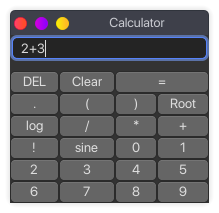
\includegraphics[width=0.45\textwidth]{img/p24/ss1.png}
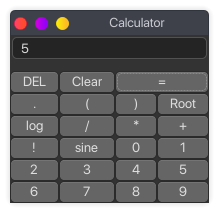
\includegraphics[width=0.45\textwidth]{img/p24/ss2.png}\newline
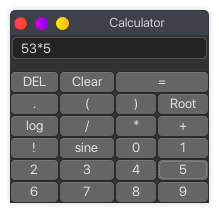
\includegraphics[width=0.45\textwidth]{img/p24/ss3.png}
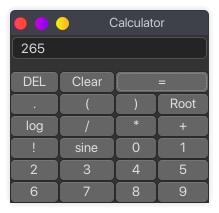
\includegraphics[width=0.45\textwidth]{img/p24/ss4.png}\newline

\subsection{Result}
The above program is run and the output is verified
\end{document}